\documentclass{beamer}
\usepackage{beamerthemelined} 
\usepackage{amsmath}
\usepackage{mathtools}
\usepackage{listings}
\usepackage{graphicx}
\usepackage{epstopdf}

\setbeamertemplate{footline}[frame number]

\lstdefinestyle{customc}{
  belowcaptionskip=1\baselineskip,
  breaklines=true,
  frame=L,
  xleftmargin=\parindent,
  language=C++,
  showstringspaces=false,
  basicstyle=\footnotesize\ttfamily,
  keywordstyle=\bfseries\color{green!40!black},
  commentstyle=\itshape\color{purple!40!black},
  identifierstyle=\color{blue},
  stringstyle=\color{orange},
}

%\usepackage{ stmaryrd }

%\usetheme{Boadilla} % Pretty neat, soft color.
%\usetheme{default}
%\usetheme{Warsaw}
%\usetheme{Bergen} % This template has nagivation on the left
%\usetheme{Frankfurt} % Similar to the default 
%with an extra region at the top.
%\usecolortheme{seahorse} % Simple and clean template
%\usetheme{Darmstadt} % not so good
% Uncomment the following line if you want %
% page numbers and using Warsaw theme%
 %\setbeamertemplate{footline}[page number]
%\setbeamercovered{transparent}
\setbeamercovered{invisible}
% To remove the navigation symbols from 
% the bottom of slides%
\setbeamertemplate{navigation symbols}{} 
%

\usepackage{graphicx}
%\usepackage{bm}         % For typesetting bold path (not \mathbold)
%\logo{\includegraphics[height=0.6cm]{yourlogo.eps}}
%
\title[Dataparallel Programming on GPUs]{Dataparallel Programming on GPUs}
\author{Daniel Rembold, Maximillian Scholz}
\institute[TUHH]
{
Technische Universit{\"a}t Hamburg Harburg \\
\medskip
{\emph{daniel.rembold@tuhh.de , maximillian.scholz@tuhh.de}}
}
\date{\today}
% \today will show current date. 
% Alternatively, you can specify a date.
%


\graphicspath{%
    {converted_graphics/}% inserted by PCTeX
    {/}% inserted by PCTeX
}
\begin{document}
\renewcommand{\figurename}{Abbildung}
%
\begin{frame}
\titlepage
\end{frame}
%

\begin{frame}
\frametitle{Inhaltsverzeichnis}

\begin{enumerate}
		\item Aufgabenstellung \\

	      	\item Einfache Implentierung \\
	      	
	      	\item NVIDIA-Template   \\ 
	      		
	      	\item Optimierung  \\ 
	  
	      	\item Laufzeit- und Performancemessung \\

		\item Fazit
\end{enumerate}

\end{frame}

%%%%%%%%%%%%%%%%%%%%%%%%%%%%%%%%%% BEGIN INTRODUCTION %%%%%%%%%%%%%%%%%%%%%%%%%%%%%%%%%
\section{Aufgabenstellung}

\begin{frame}
\frametitle{Aufgabenstellung}

\begin{itemize}
\item
M\"oglichst effiziente Implementierung einer Matrixmultiplikation in row-major und column-major Format 

\item
Quadratische Matrizen der Dimension $32 * k , k \in \{ 1,2,4,\dots,128 \} $ 
\end{itemize}







\end{frame}

%%%%%%%%%%%%%%%%%%%%%%%%%%%%%%%%%%%%%%%%%%%%%%%%%%%%

\section{Einfache Implentierung}



%%%%%%%%%%%%%%%%%%%%%%%%%%%%
\begin{frame}[fragile]
\frametitle{Naiver Algoritmus}

\begin{itemize}
\item C-Code f\"ur die CPU 
\item Sequentielle Ausf\"uhrung
\end{itemize}

\begin{lstlisting}[style=customc,caption=Matrixmultiplication in C]
int i,j,k;

for( i = 0, i<Ndim; i++){
  for( j = 0, j<Mdim;j++){
    for( k = 0; k<Pdim; k++){
      C[i*Ndim+j] += A[i*Ndim+k] * B[k*Pdim+j]; 
    }
  }
}
\end{lstlisting}



\end{frame}


% % % % % % % % % % % % % % % % % % % % % % % % % % % % %

\begin{frame}[fragile]
\frametitle{Einfache Implementierung}
 
Einfache Implementierung in OpenCL
\begin{lstlisting}[style=customc,caption=Einfachster Code in OpenCL]
int i,j,k;
i = global_id(0);
j = global_id(1);
  for(k=0; k<Pdim; k++){
    C[i*Ndim+j] += A[i*Ndim+k] * B[k*Pdim+j]; 
  }
\end{lstlisting}


\end{frame}

\begin{frame}
\frametitle{Laufzeit}
\begin{center}
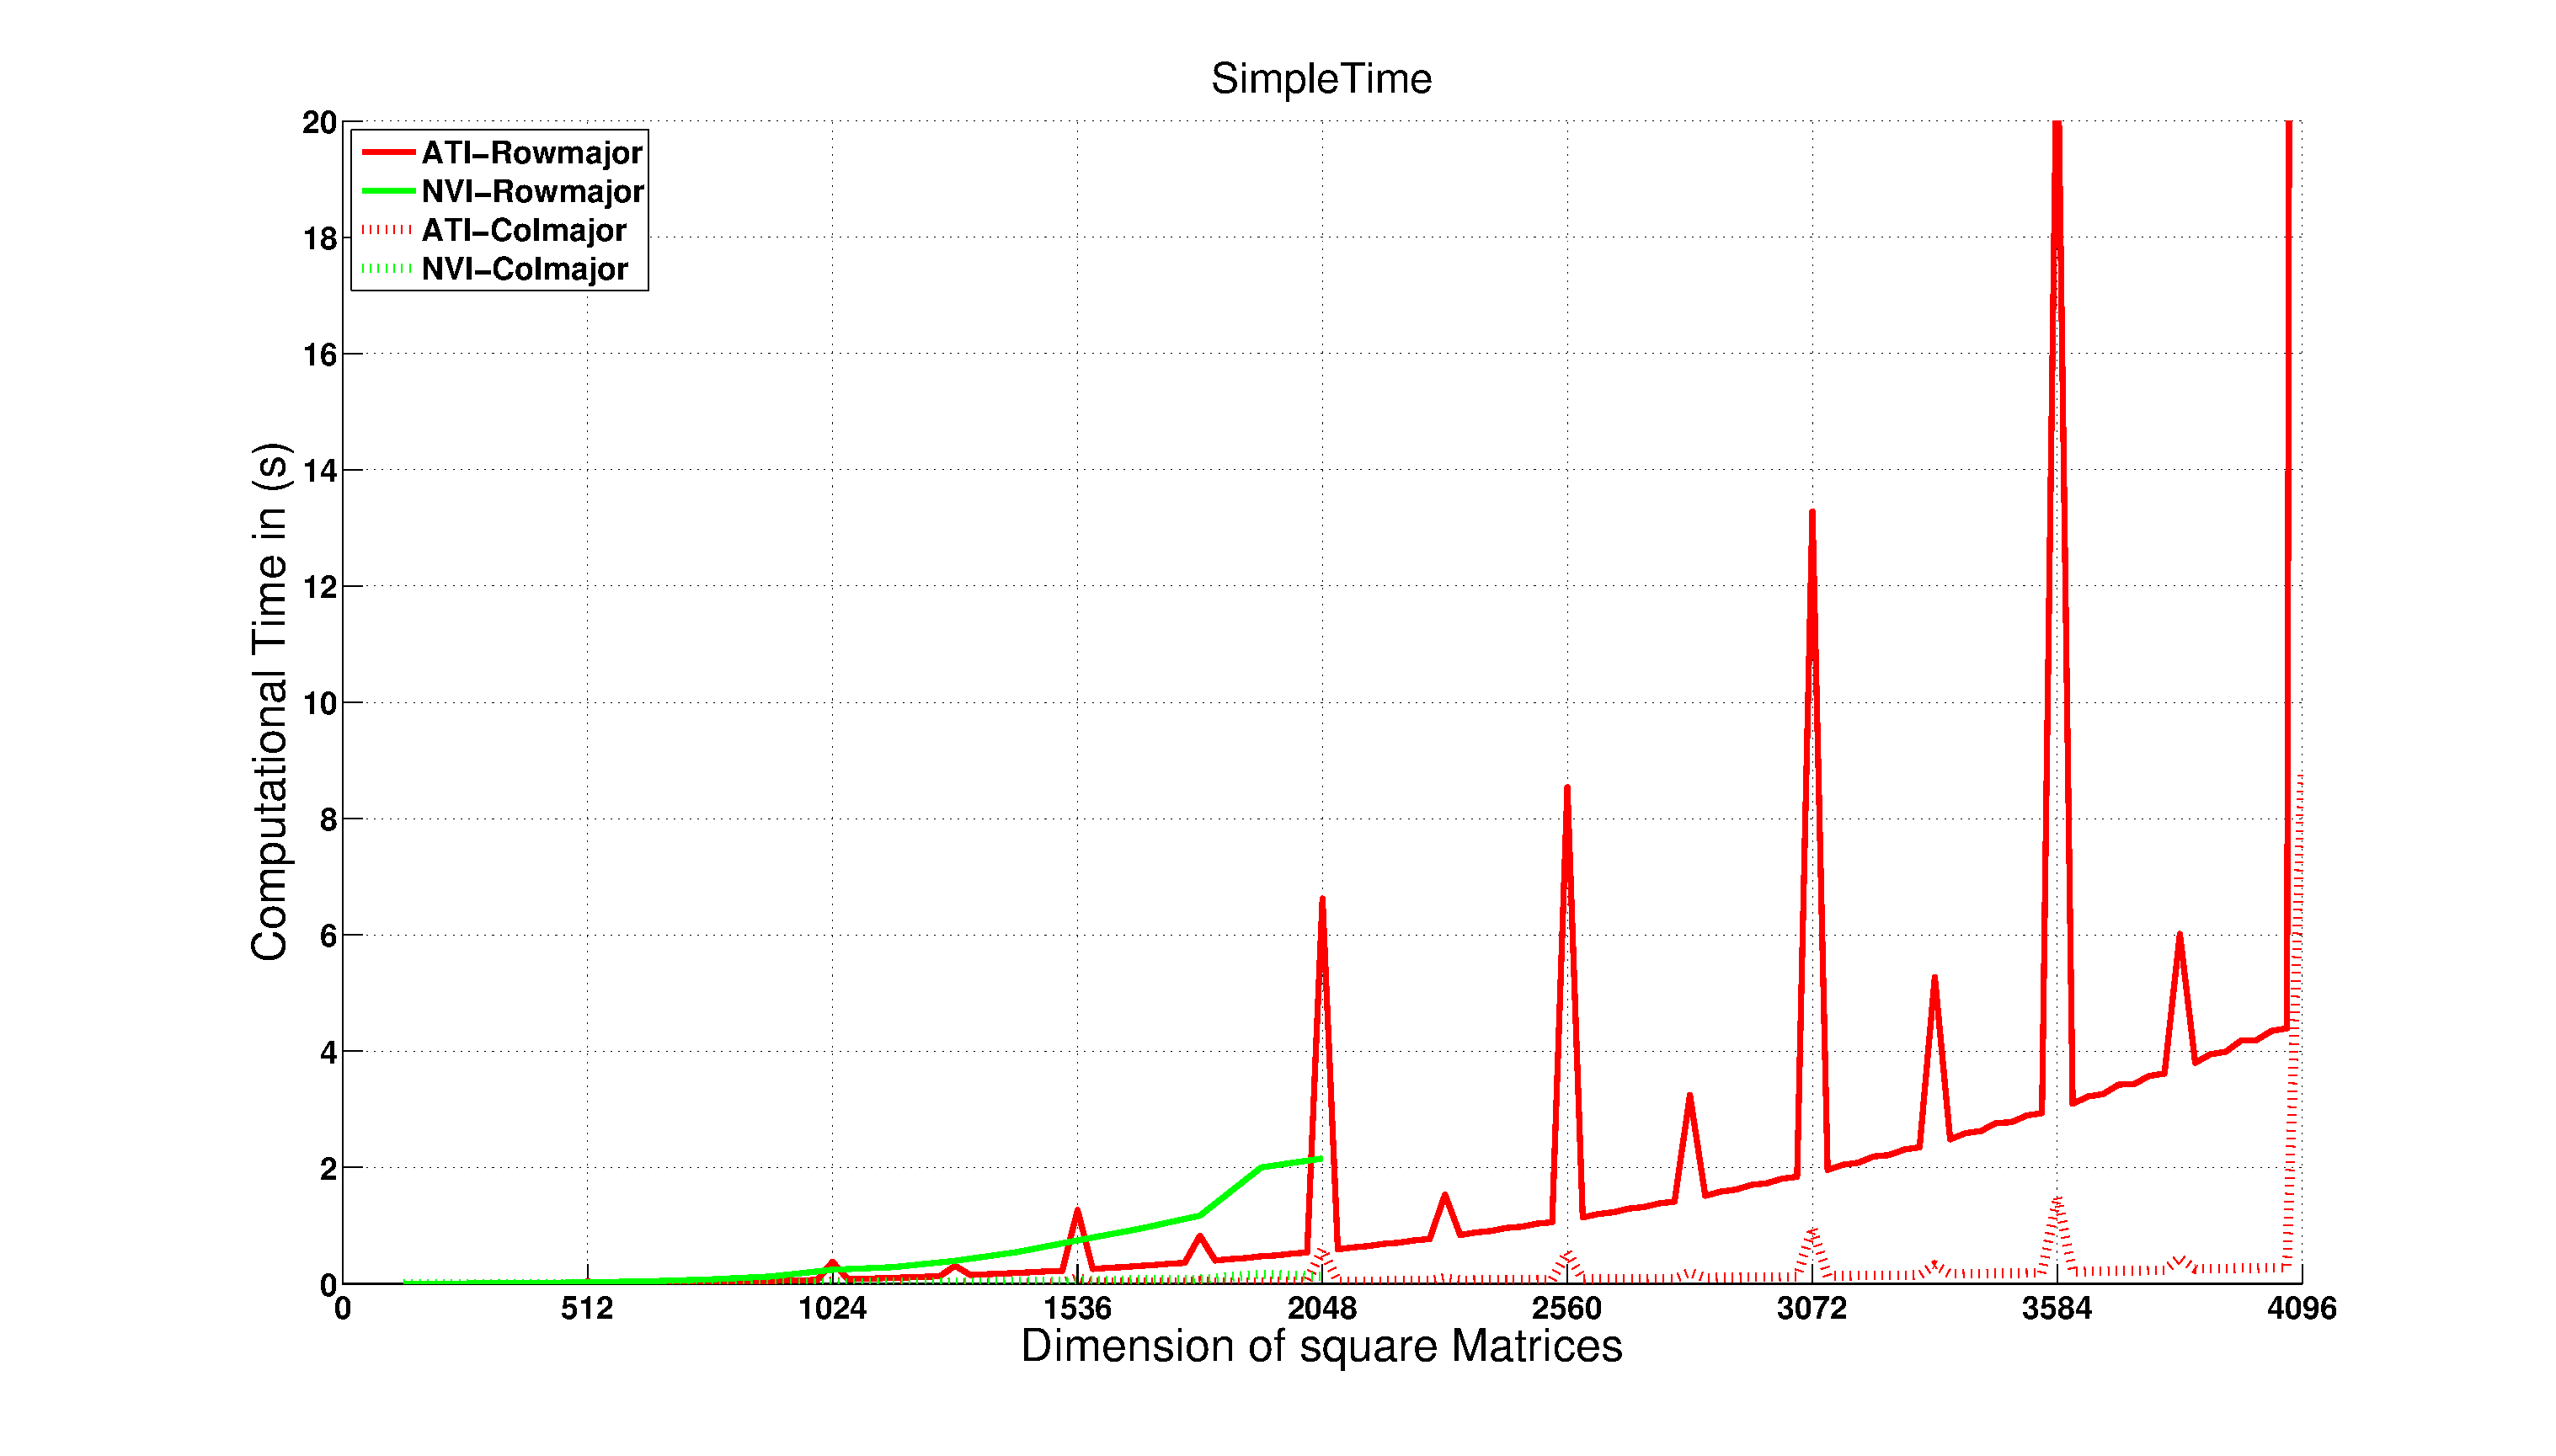
\includegraphics[width=12.5cm]{SimpleTime}
\end{center}

	
\end{frame}

\begin{frame}
	\frametitle{Performance}
\begin{center}
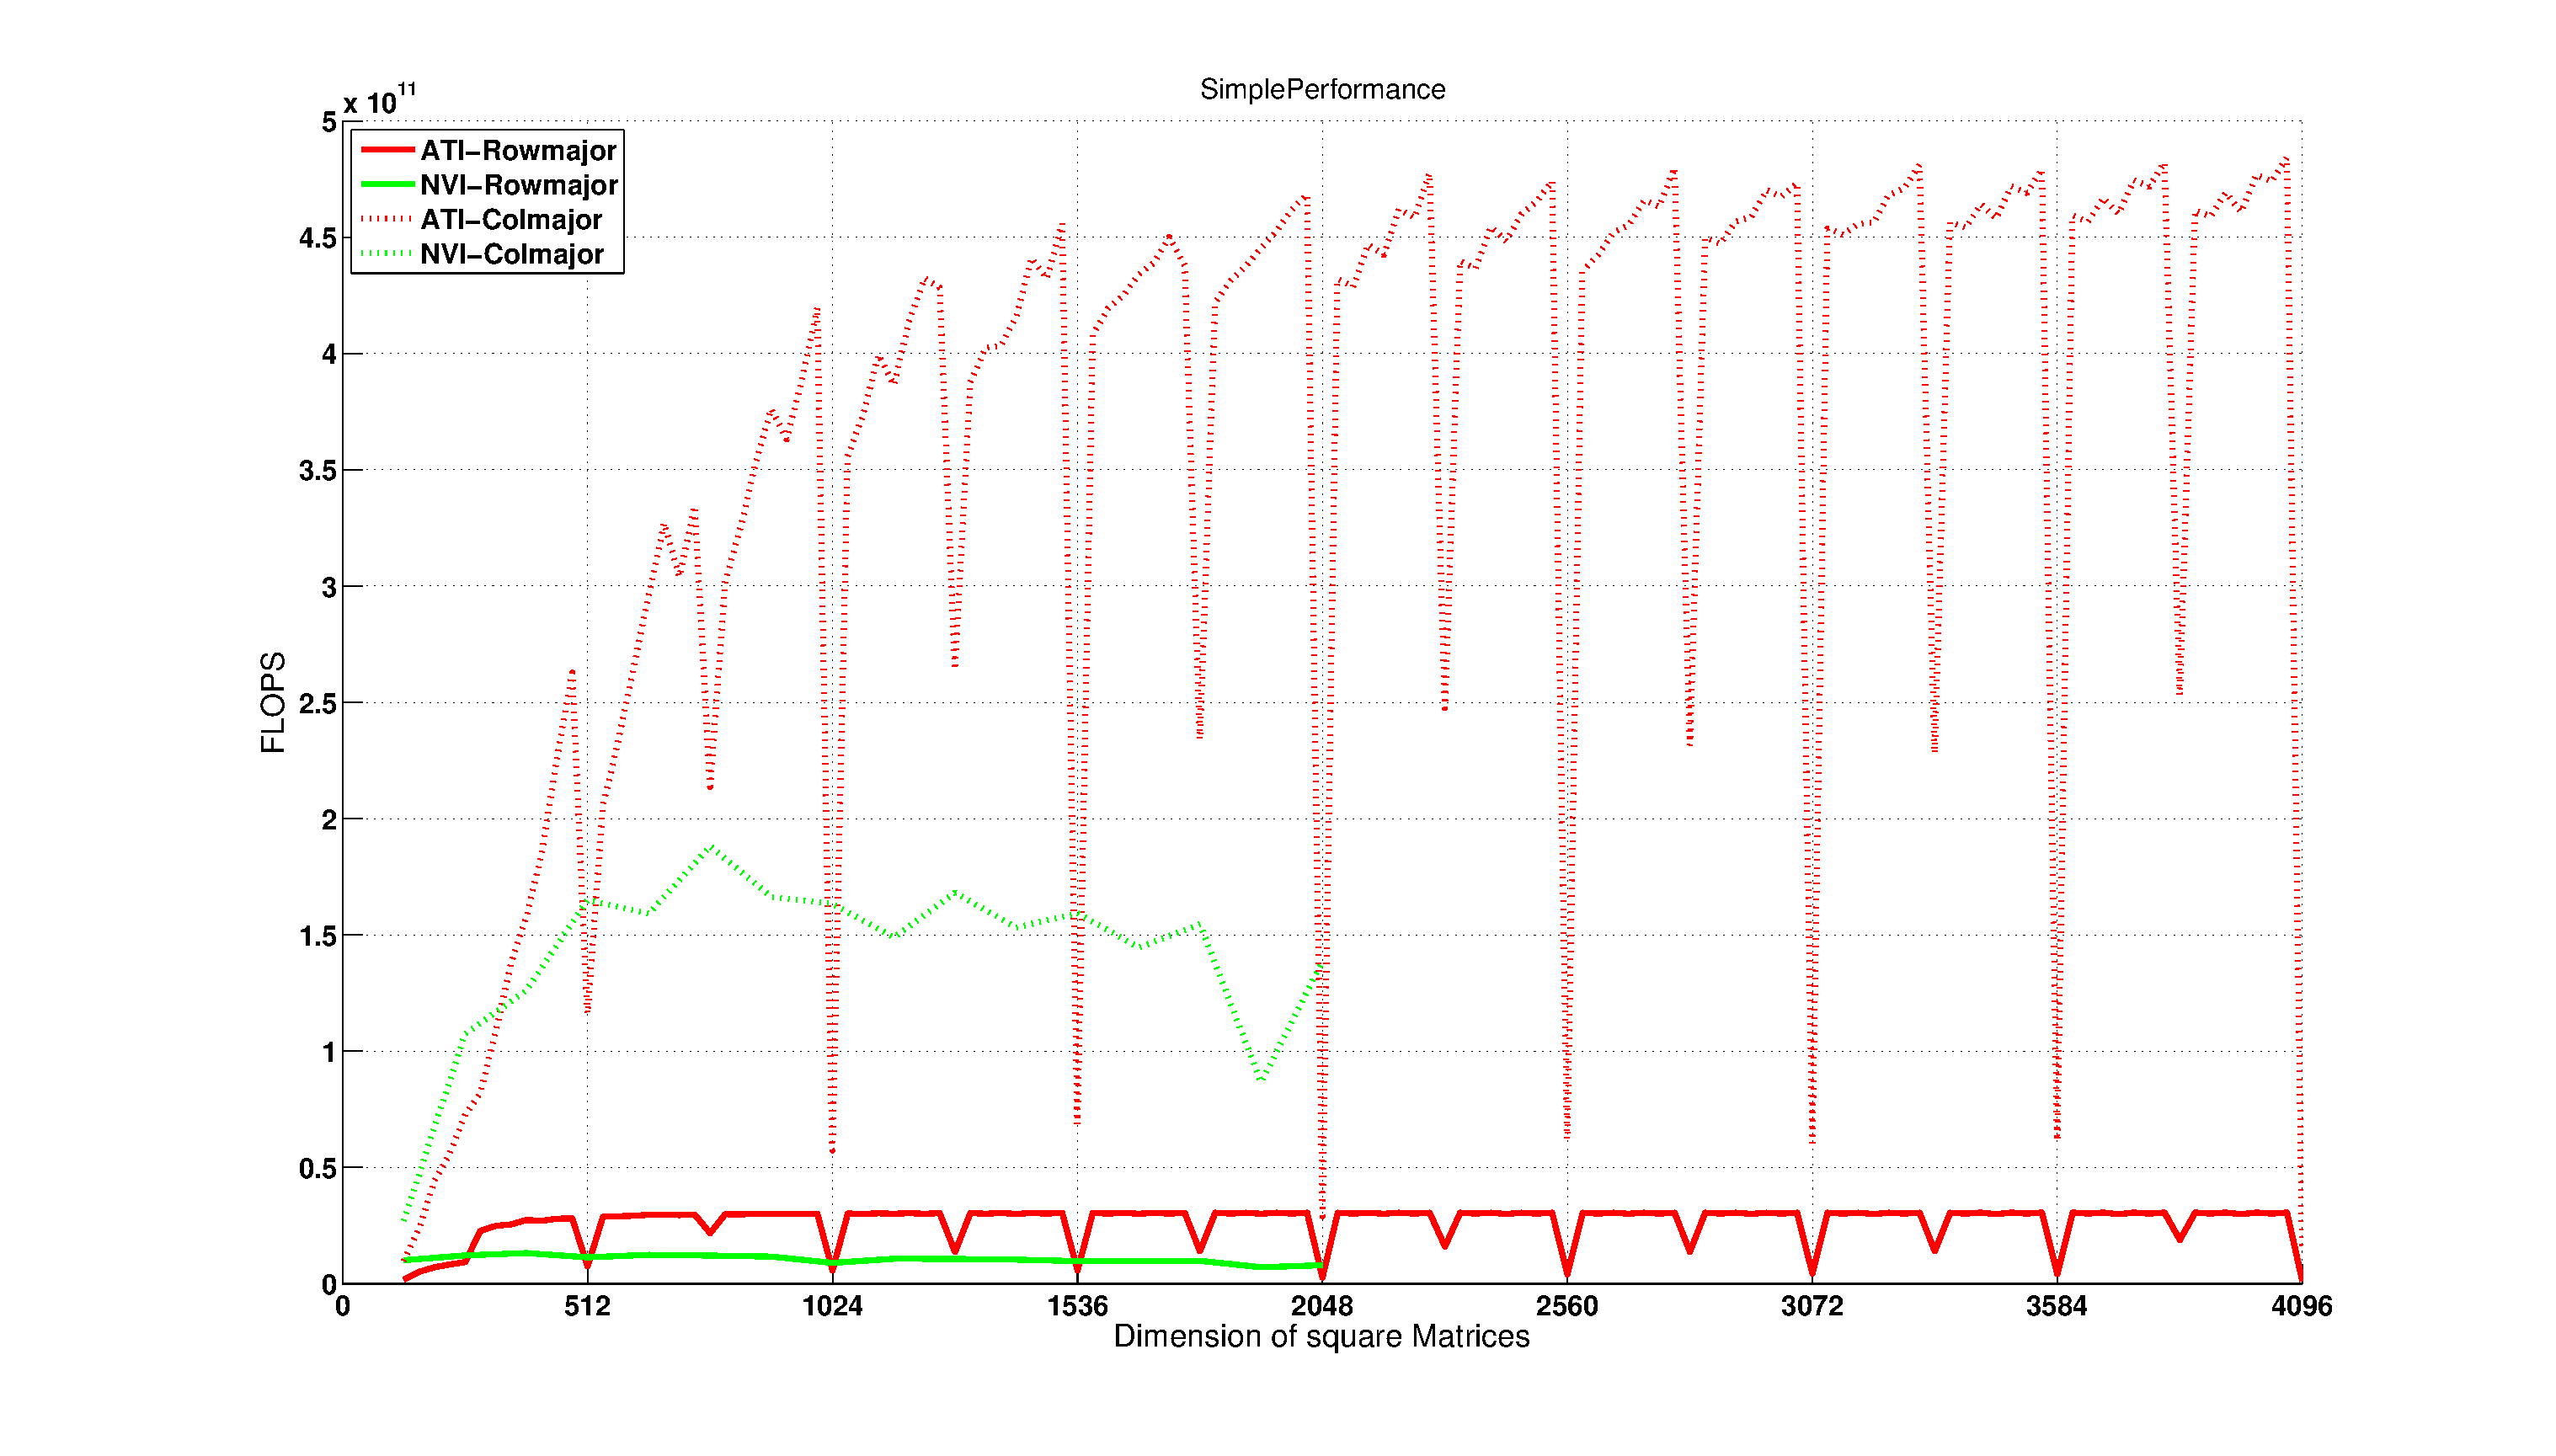
\includegraphics[width=12.5cm]{SimplePerformance}
\end{center}


	
\end{frame}
%%%%%%%%%%%%%%%%%%%%%%%%%%%

% % % % % % % % % %  % %  % % %  % % % %  % %%  % % %  

\section{NVIDIA-Template}
\begin{frame}[fragile]
\frametitle{NVIDIA-Template}

\begin{itemize}
\item
Zerlegung der Matrix in Bl\"ocken
\item
Verwendung von lokalem Speicher 
\end{itemize}

\begin{lstlisting}[style=customc,caption=NVIDIA-Snippet]
int bx = get_group_id(0); // Blockindex x
int by = get_group_id(1); // Blockindex y
int tx = get_local_id(0); // Threadindex x
int ty = get_local_id(1); // Threadindey y
\end{lstlisting}


%TODO Laufzeitmessung hochladen abh. von Blockgröße

\end{frame}

%  % %  % % % % % % % % % %  % % %

\begin{frame}[fragile]
\begin{lstlisting}[style=customc,caption=NVIDIA-Snippet(2)]
__local T As[16][16];__local T Bs[16][16]; T Csub = 0.0f;
for (int a = aBegin, b = bBegin; a <= aEnd; a += aStep, b += bStep){ 
	As[ty][tx] = A[a + ty + hA * tx];
	Bs[ty][tx] = B[b + ty + hA * tx];
	barrier(CLK_LOCAL_MEM_FENCE);
		for (int k = 0; k < 16; ++k)Csub += As[ty][k] * Bs[k][tx];
		}
    barrier(CLK_LOCAL_MEM_FENCE);
}
int c = 16 * ( by + hA* bx):
C[c + hA * tx + ty] = Csub;
\end{lstlisting}


\end{frame}



\section{Optimierung}
\begin{frame}[fragile]
\frametitle{Optimierung}

\begin{itemize}
\item
Anzahl der Threadblocks werden verringert, Anzahl der Blocks bleiben
\item
Halb so viele Threads, jedoch doppelt so viel Arbeit pro Thread
\end{itemize}


\begin{lstlisting}[style=customc,caption=Optimized Code in OpenCL]
T Csub[2] = {0,0};
 __local T As[BLOCK_SIZE][BLOCK_SIZE]; 
 __local T Bs[BLOCK_SIZE][BLOCK_SIZE]; 
for (int a = aBegin, b = bBegin; a <= aEnd;a += aStep, b+=bStep){ 
	AS(ty, tx) = A[a + wA * ty + tx]; 
	BS(ty, tx) = B[b + wB * ty + tx]; 
	AS(ty+16, tx) = A[a + wA * (ty+16) + tx]; 
	BS(ty+16, tx) = B[b + wB * (ty+16) + tx]; 
	barrier(CLK_LOCAL_MEM_FENCE); // sync threads
}
\end{lstlisting}



\end{frame}


\begin{frame}[fragile]
\frametitle{Optimierung}
\begin{lstlisting}[style=customc,caption=innere Schleife und Output]
for (int k = 0; k < BLOCK_SIZE; ++k){ 
	Csub[0] += AS(ty, k) * BS(k, tx); 
	Csub[1] += AS(ty+16, k) * BS(k, tx); 
} 
barrier(CLK_LOCAL_MEM_FENCE); // sync threads
} 
int c = wB * BLOCK_SIZE * by + BLOCK_SIZE * bx; 
C[c + wB * ty + tx] = Csub[0]; 
C[c + wB * (ty+16) + tx] = Csub[1]; 
\end{lstlisting}

\begin{itemize}

\item
Daten aus dem lokalen Speicher werden wiederverwendet
\item 
Weniger Threads pro Block erm\"oglich \"Uberlappung von Speicherzugriff mit Arithmetik
\end{itemize}


\end{frame}

\section{Laufzeit- und Performancemessung}
\begin{frame}
\frametitle{Laufzeitmessung auf ATI und NVIDIA}
\begin{center}
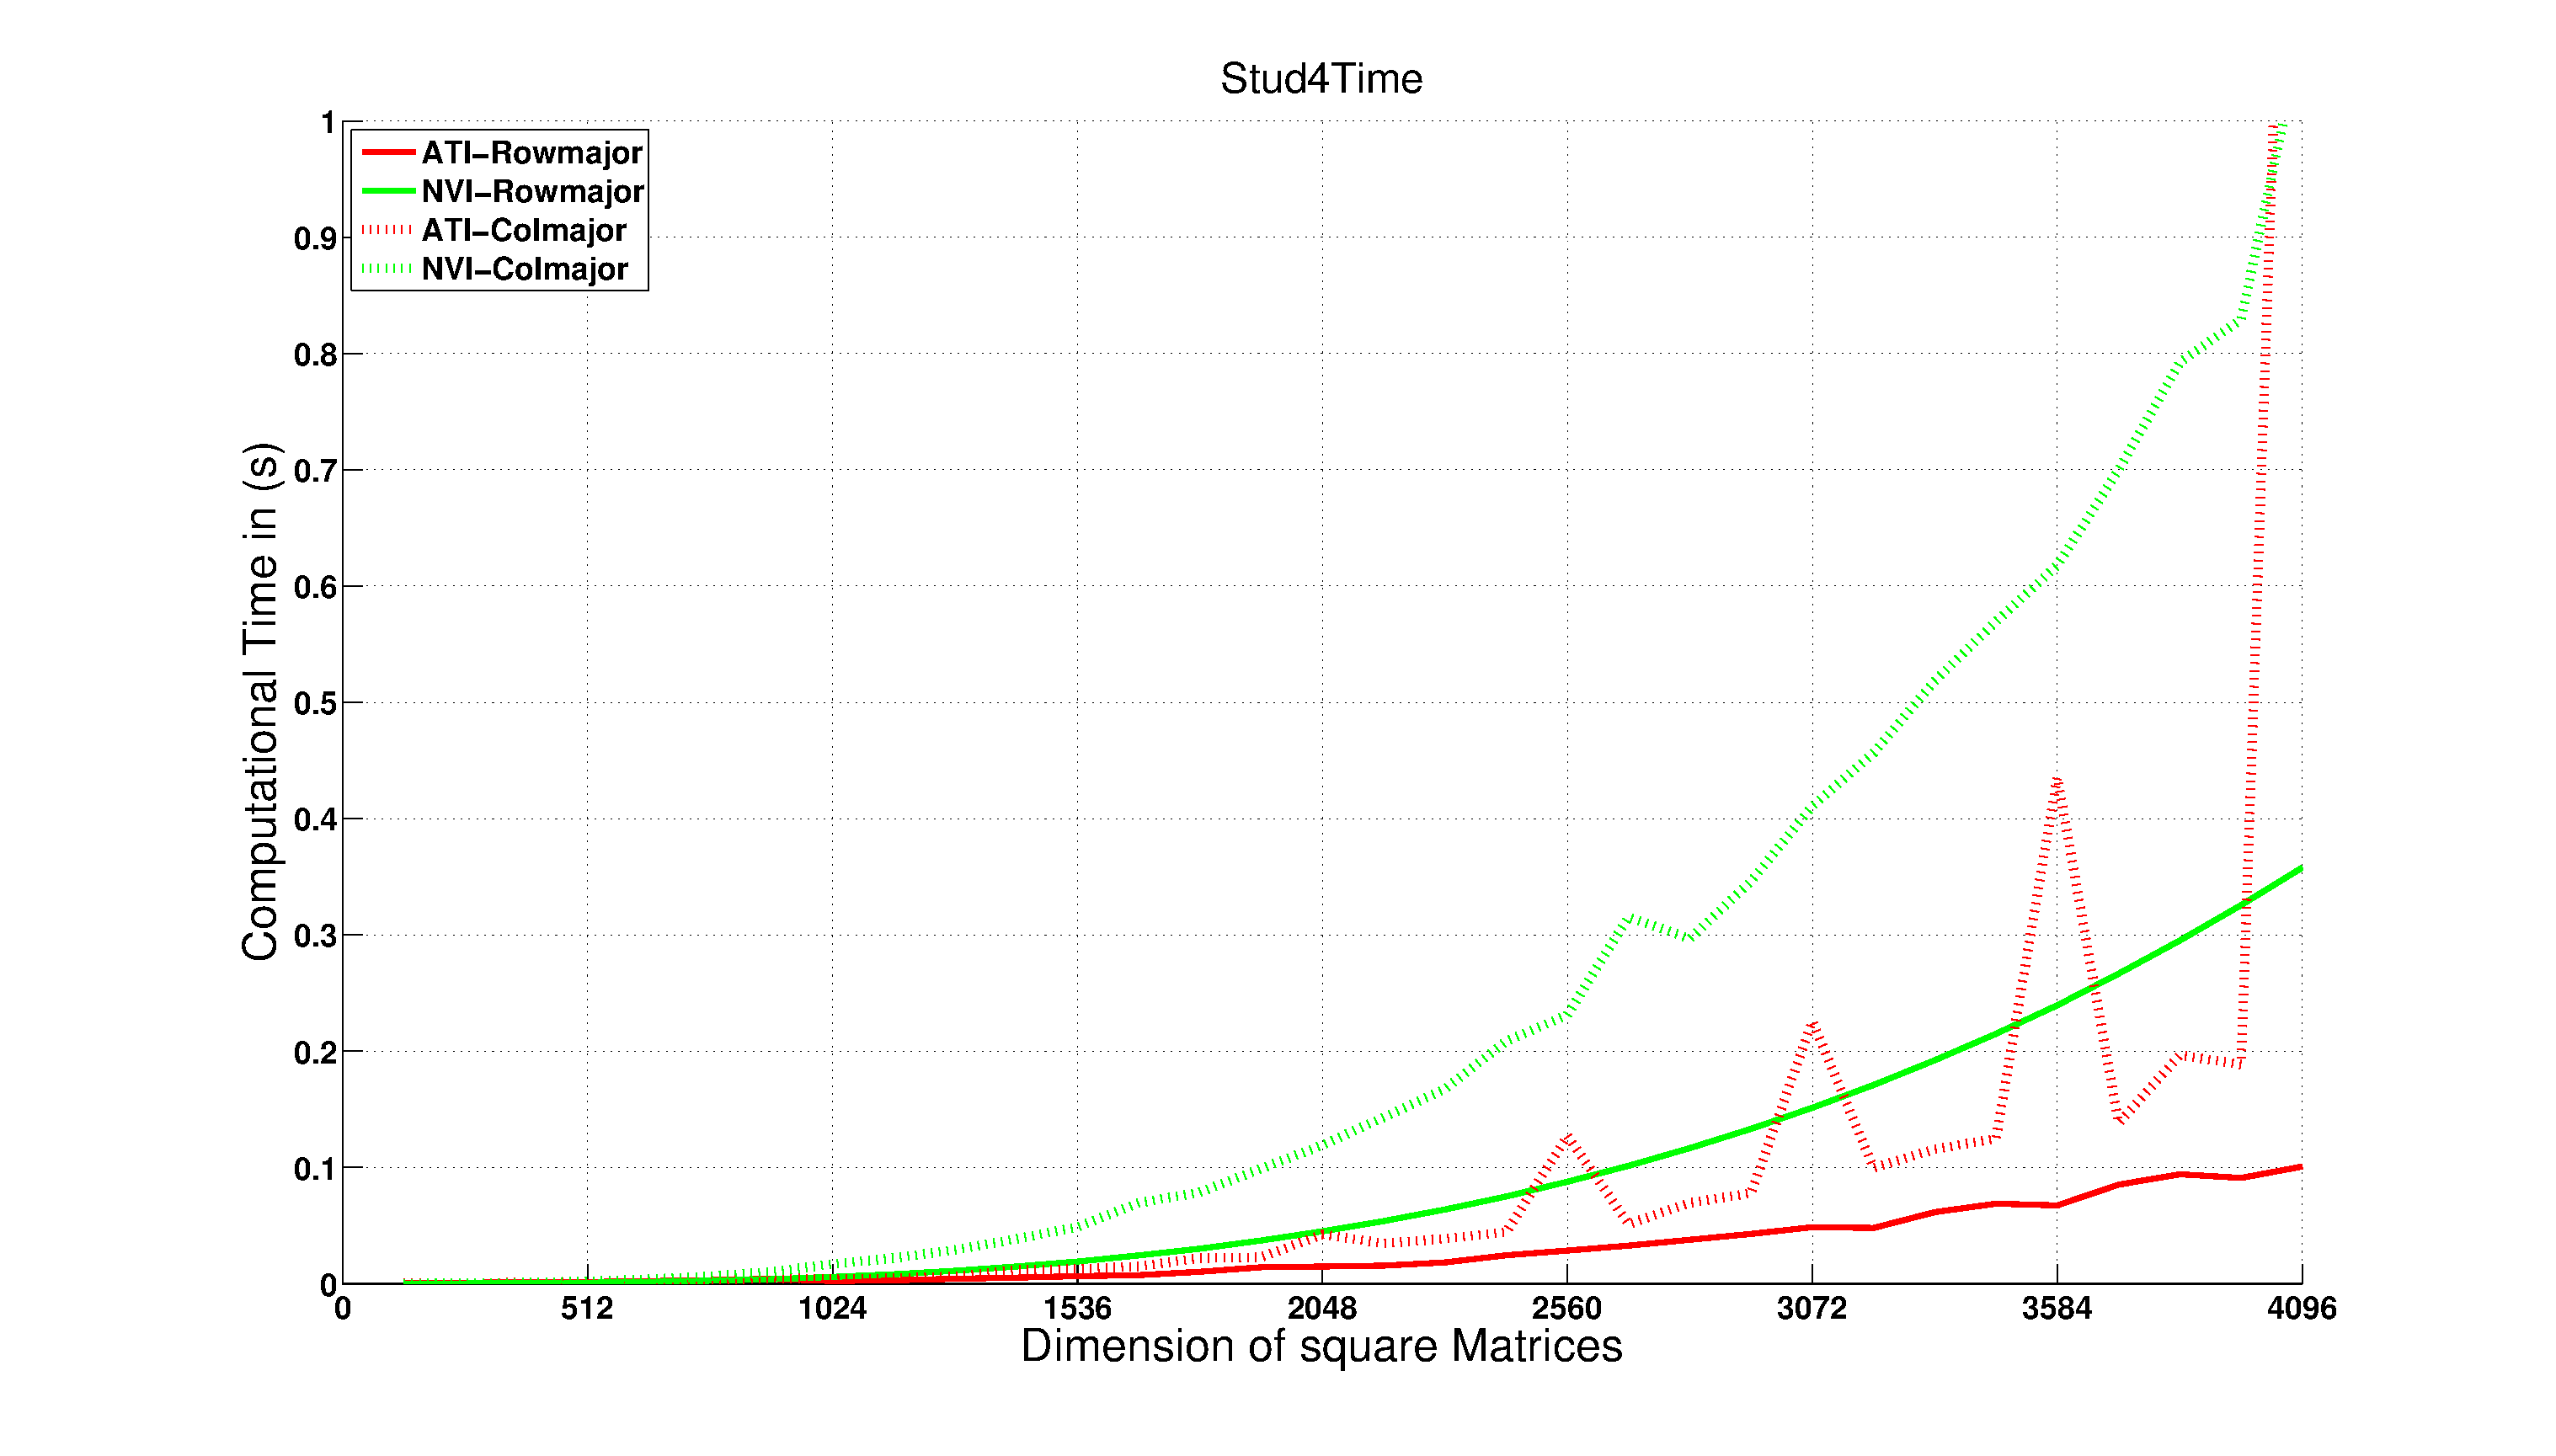
\includegraphics[width=12.5cm]{Stud4Time}
\end{center}

\end{frame}

\begin{frame}
\frametitle{Performancemessung auf ATI und NVIDIA}
\begin{center}
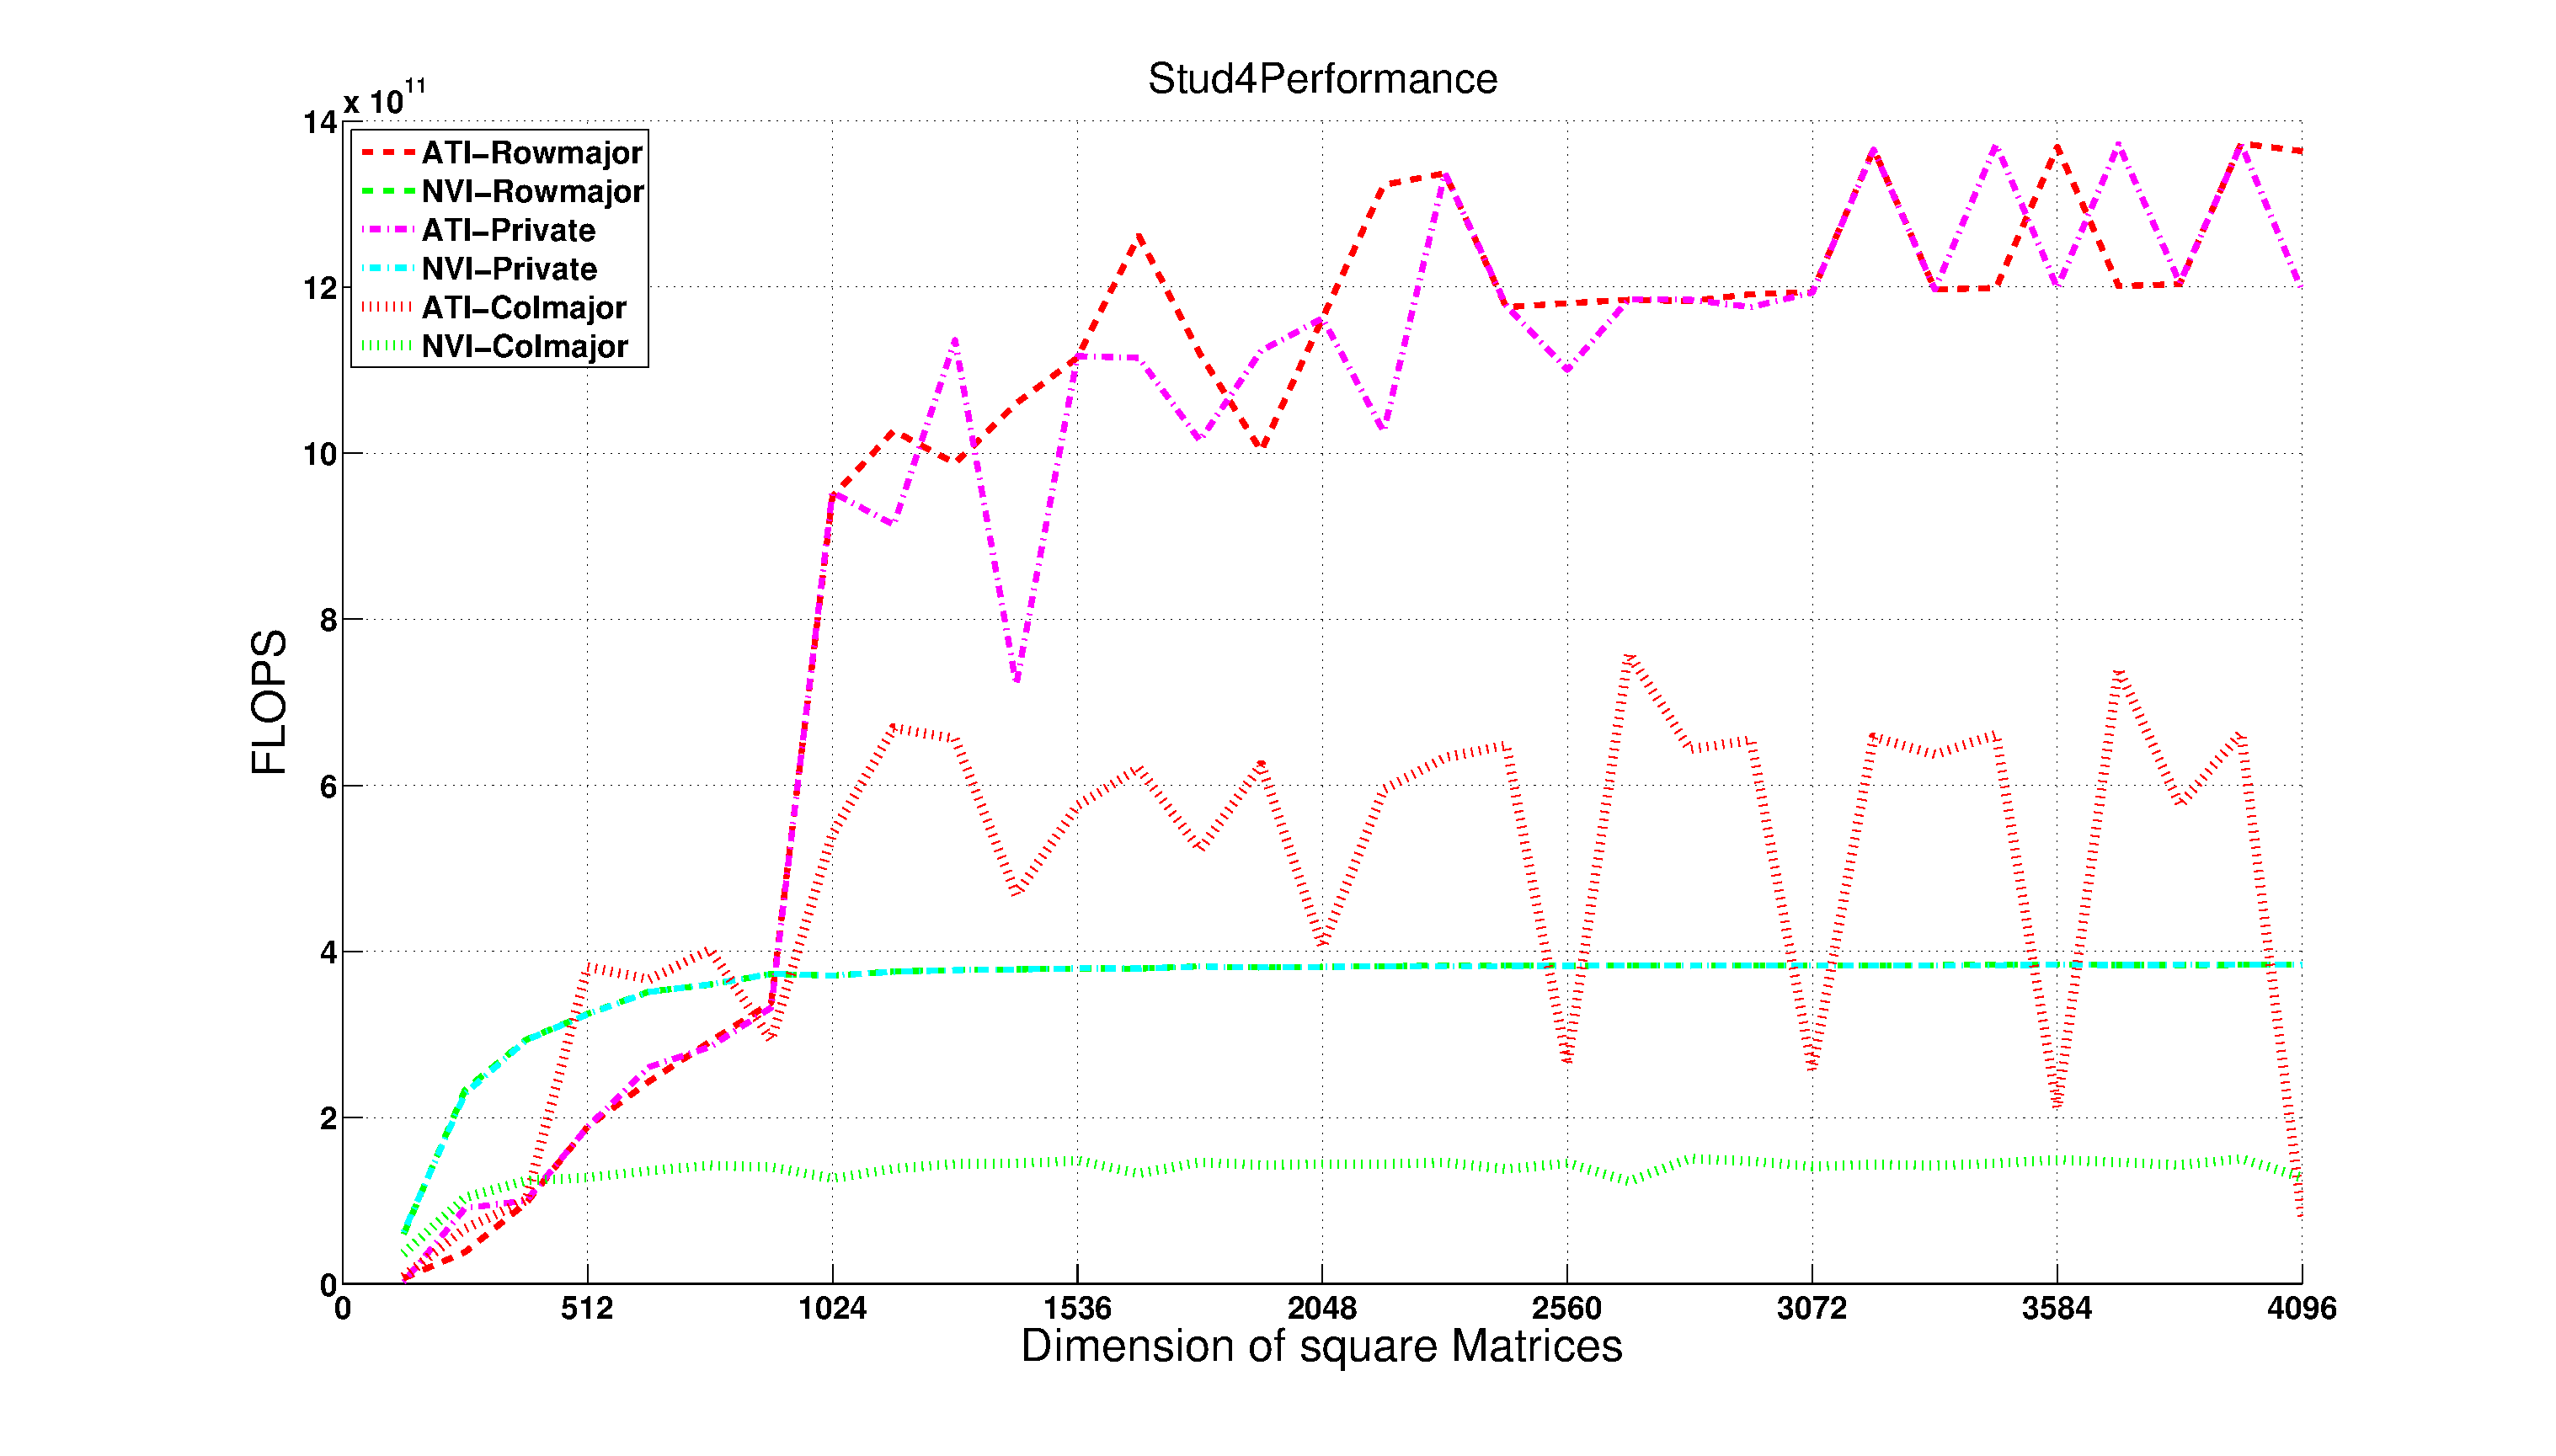
\includegraphics[width=12.5cm]{Stud4Performance}
\end{center}

\end{frame}


\section{Fazit}

\begin{frame}
\frametitle{Vergleich}

\begin{tabular}{|l|l|l|l|l|l|}
	\hline  & Simple Perf. & Opt. Perf. & Peak Perf. & S/P & O/P \\ 
	\hline AMD RM & $3.056e+10$ & $1.372e+12$ & $3.79e+12$ & 0.8 & 36.23 \\ 
	\hline AMD CM & $4.843e+11$ & $7.588e+11$ & $3.79e+12$ & 12.78 & 20.03 \\ 
	\hline Nvidia RM & $ 1.319e+10$ & $3.845e+11$ & $1.03e+12$ & 1.28 & 37.33 \\ 
	\hline Nvidia CM & $ 1.881e+11$ & $1.506e+11$ & $1.03e+12$ & 18.26 & 14.63 \\ 
	\hline 
	\end{tabular} 
	
\end{frame}


\begin{frame}
\frametitle{Begr\"undung der Ergebnisse und m\"ogl. Verbesserungen}

\begin{itemize}
\item Vektorarithmetik (float4)
\item Image-Objekte
\end{itemize}

 
\end{frame}













%%%%%%%%%%%%%%%%%%%%%%%%%%%%%%%%%
%%%%%%%%%%%%%%%%%%%%%%%%%%%%%%%%%
%%%%%%%%%%%%%%%%%%%%%%%%%%%%%%%%%

\begin{frame}
\frametitle{Quellen}


\footnotesize{
\begin{thebibliography}{99}
 \bibitem[Label1, 2010]{key1} University of Bristol
 \newblock Optimizing OpenCL performance
 \newblock \url{http://www.cs.bris.ac.uk/home/simonm/workshops/OpenCL_lecture3.pdf} 
\end{thebibliography}
}



\footnotesize{
\begin{thebibliography}{99}
 \bibitem[Label1, 2010]{key1}NVIDIA 
 \newblock OpenCL SDK Code Samples
 \newblock \url{https://developer.nvidia.com/opencl} 
\end{thebibliography}
}


\footnotesize{
\begin{thebibliography}{99}
 \bibitem[Label1, 2010]{key1} Vasily Volkov
(UC Berkeley , September 22, 2010)
 \newblock Better Performance at Lower Occupancy 
 \newblock \url{http://www.cs.berkeley.edu/~volkov/volkov10-GTC.pdf} 
\end{thebibliography}
}





\end{frame}
 
 
 
\begin{frame}
\centerline{Vielen Dank f{\"u}r eure Aufmerksamkeit!}
\end{frame}
% End of slides
\end{document}
